\input ../SlidePreamble
\input ../preamble

\begin{document}

{\Huge

  \centerline{\bf TTIC 31230, Fundamentals of Deep Learning}
  \bigskip
  \centerline{David McAllester, Autumn 2023}


  \vfill
  \centerline{\bf AlphaZero, MuZero and AlphaStar}
  \vfill
  \vfill          

\slide{AlphaGo Fan (October 2015)}

AlphaGo Defeats Fan Hui, European Go Champion.

\vfill
\centerline{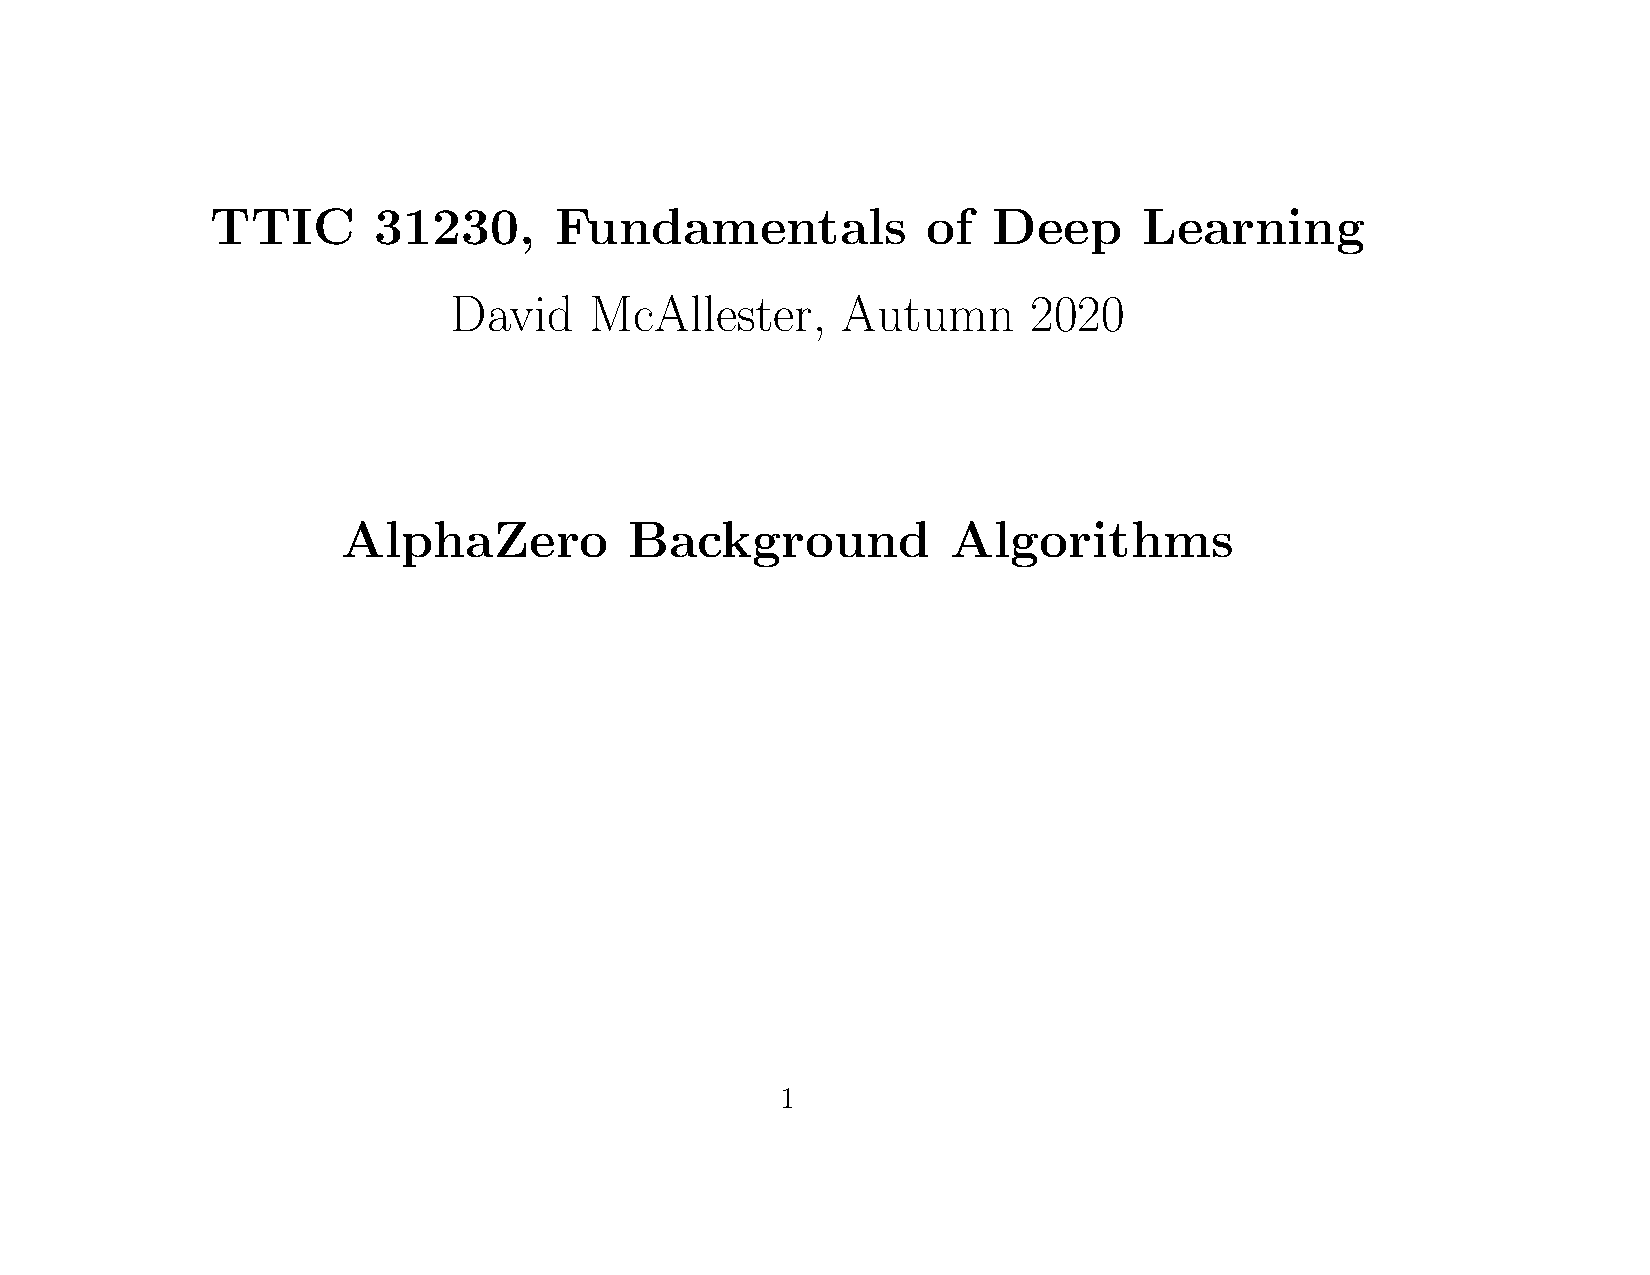
\includegraphics[width=4in]{\images/alphago}}

\slide{AlphaGo Lee (March 2016)}

\vfill
\centerline{\includegraphics[width=8in]{\images/alphagolee}}

\slide{AlphaGo Zero vs. Alphago Lee (April 2017)}

{\bf AlphaGo Lee:}

\begin{itemize}
\item Trained on both human games and self play.
  
\item Trained for Months.

\item Run on many machines with 48 TPUs for Lee Sedol match.
\end{itemize}

{\bf AlphaGo Zero:}
\begin{itemize}
\item Trained on self play only.
  
\item Trained for 3 days.

\item Run on one machine with 4 TPUs.

\item Defeated AlphaGo Lee under match conditions 100 to 0.
\end{itemize}

\slide{AlphaZero Defeats Stockfish in Chess (December 2017)}

AlphaGo Zero was a fundamental algorithmic advance for general RL.

\vfill
The general RL algorithm of AlphaZero is essentially the same as that of AlphaGo Zero.


\slide{}

\centerline{\bf Some Background}

\vfill

\slide{Early Computer Chess}

First computer chess algorithm (min-max tree search) --- Claude Shannon, 1949

\vfill
$\alpha$-$\beta$ pruning --- various originators (including John McCarthy) circa 1960.

\vfill
$\alpha$-$\beta$ pruning was the backbone of all computer chess before AlphaGo 2015.

\vfill
The game of Go is clearly not approachable by these methods.

\slidetwo{Monte-Carlo Tree Search (MCTS)}
{Brugmann (1993)}

First major advance in computer Go.

\vfill
To estimate the value of a position (who is ahead and by how much)
run a cheap stochastic policy to generate a sequence of moves (a rollout) and see who wins.

\vfill
Select the move with the best rollout value.

\slidetwo{(One Armed) Bandit Problems}
{Robbins (1952)}

Bandit problems were studied in an independent line of research.

\vfill
Consider a set of choices.  The standard example is a choice between different slot machines with different but unknown expected payout.
The ``phrase one-armed bandit'' refers to a slot machine.

\vfill
But another example of choices might be the moves in a game.

\slide{Bandit Problems}

\vfill
Consider a set of choices where each choice gets a stochastic reward.

\vfill
We can select a choice and get a reward as often as we like.

\vfill
We would like to determine which choice is best using a limited number of trials.

\slidetwo{The Upper Confidence Bound (UCB) Algorithm}
{Lai and Robbins (1985)}

For each action choice (bandit) $a$, construct a confidence interval for its average reward
based on $n$ trials for that acrtion.

\vfill
$$\mu(a) \in \hat{\mu}(a) \pm 2\sigma(a)/\sqrt{n(a)}$$

\vfill
Always select

$$\argmax_a \;\; \hat{\mu}(a) + 2\sigma(a)/\sqrt{n(a)}$$

\slidetwo{The Upper Confidence Tree (UCT) Algorithm}
{Kocsis and Szepesvari (2006), Gelly and Silver (2007)}

The UCT algorithm grows a tree by running ``simulations''.

\vfill
Each simulation descends into the tree to a leaf node, expands that leaf, and returns a value.

\vfill
In the UCT algorithm each move choice at each position is treated as a bandit problem.

\vfill
We select the child (bandit) with the lowest upper bound as computed from simulations selecting that child.


\slidetwo{Bootstrapping from Game Tree Search}
{Vaness, Silver, Blair and Uther, NeurIPS 2009}

In bootstrapped tree search we do a tree search to compute a min-max value $V_{\mathrm{mm}}(s)$
using tree search with a static evaluator $V_\Phi(s)$.  We then try to fit the static value to the min-max value.

\vfill
$$\Delta \Phi = - \eta \nabla_\Phi \left(V_\Phi(s) - V_{\mathrm{mm}}(s)\right)^2$$

\vfill
This is similar to minimizing a Bellman error between $V_\Phi(s)$ and a rollout estimate of the value of $s$ but where the rollout
estimate is replaced by a min-max tree search estimate.


\slide{The Value and Policy Networks}

The major innovation of AlphaGo and AlphaZero is to use CNNs as evaluation functions.

\vfill
We have a policy network computing $\pi_\Phi(a|s)$ and a value network computing $V_\Phi(s)$.

\slide{The Value and Policy Networks}

\centerline{$\pi_\Phi(a|s)$ \hspace{.5in} $V_\Phi(s)$}
\centerline{\includegraphics[height=3.0in]{\images/alphagoArchitecture2}}

\vfill
In AlphaZero the networks are either 20 block or 40 block ResNets and either separate networks or one dual-headed network.

\slide{Tree Search Algorithm}

Move selection involves a tree search.

\vfill
Each node represents a board position $s$ and stores the following information.

\vfill
\begin{itemize}
\item $V_\Phi(s)$ --- the value network value for the position $s$.
\vfill
\item The policy probabilities $\pi_\Phi(a|s)$ for each legal action $a$
from that position.
\vfill
\item An initially empty set of children nodes.
\end{itemize}


\slide{Tree Search Algorithm}

\vfill
The tree is grown by a series of ``simulations''.

\vfill
Each simulation starts at the root and recursively selects a move.

\vfill
The selected move $a$ from state $s$ may or may not correspond to an existing child of $s$.

\vfill
If the child exists the simulation continues down that path.

\vfill
If the child does not exist a new child node is created for the selected move and the simulation terminates.

\vfill
Each simulation adds one new leaf $s$ and returns the value $V_\Phi(s)$ to all parents of $s$ in the tree.

\slide{Tree Search Algorithm}

In addition to $V_\Phi(s)$, $\pi_\Phi(a|s)$ and set of children nodes, each node $s$ contains
the following for each possible action $a$.

\vfill
\begin{itemize}
\item The number $N(s,a)$ of simulations that have tried move $a$ from $s$. This is initially zero.

\vfill
\item The average $\overline{V}(s,a)$ of $V_\Phi(s)$ plus the values returned by the the simulations that selected
 move $a$ from position $s$.  This averages $1 + N(s,a)$ numbers.
\end{itemize}

\slide{Simulations and Upper Confidence Bounds}

At a node $s$ a simulation selects the move $\argmax_a \mathrm{UCB}(s,a)$ where we have

\vfill
$$\mathrm{UCB}(s,a) =   \overline{V}(s,a) + \lambda_u\; \pi_\Phi(a|s)/(1+N(s,a))$$

\vfill
We set $\lambda_u$ be large enough that $\mathrm{UCB}(s,a)$ will typically decrease as $N(s,a)$ increases.

\slide{Root Action Selection}

When the search is completed, we must select a move from the root position to make actual progress in the game.  For this we use a post-search stochastic policy

\vfill
$$\pi_{s_{\mathrm{root}}}(a) \propto N(s_{\mathrm{root}},a)^\beta$$

\vfill
where $\beta$ is a temperature hyperparameter.

\slide{Constructing a Replay Buffer}

We run a large number of games.

\vfill
We construct a replay buffer of triples $(s,\pi_{s},R)$ where

\vfill
\begin{itemize}
\item $s$ is a position encountered in a game and hence a root position of a tree search.

\vfill
\item $\pi_{s}$ is the distribution on $a$ defined by $P(a) \propto N(s,a)^\beta$.

\vfill
\item $R \in \{-1,1\}$ is the final outcome of the game for the player whoes move it is at position $s$.
\end{itemize}

\slide{The Loss Function}

\vfill
Training is done by SGD on the following loss function.

$$\Phi^*\; = \;\argmin_\Phi \;E_{(s,\pi,R) \sim \mathrm{Replay},\;a \sim \pi}\;\left(\begin{array}{l} (V_\Phi(s) - R)^2 \\ \\ - \lambda_\pi\log \pi_\Phi(a|s) \\ \\ + \lambda_R\;||\Phi||^2\end{array}\right)$$

\vfill
The replay buffer is periodically updated with new self-play games.

\slide{The AlphaZero Algorithm}

The AlphaZero algorithm is a general RL learning method.  It can be applied to any problem of sequential decision making.

\vfill
The AlphaZero algorithm is used to train AlphaProof (September 2024).


\slide{Training Time}

Single 20 block dual-headed ResNet.

\vfill
4.9 million Go games of self-play

\vfill
0.4s thinking time per move

\vfill
About 8 years of Go thinking time in training was completed in three days

\vfill
About 1000 fold parallelism.

\slide{Elo Learning Curve for Go}

\centerline{\includegraphics[height = 5in]{\images/alphalearning1}}

\slide{Learning Curve for Predicting Human Go Moves}

\centerline{\includegraphics[height = 5in]{\images/alphalearning2}}

\slide{Ablation Studies}

\centerline{\includegraphics[height=3.0in]{\images/alphagoArchitecture2}}

\vfill
We evaluate 20 layer networks which are either traditional CNNs or resnet and are either two separate networks or one network with dual heads.

\slide{Ablation Studies}

\centerline{\includegraphics[height = 5in]{\images/alphaablation}}

\slide{Increasing Blocks and Training}

Increasing the number of Resnet blocks from 20 to 40.

\vfill
Increasing the number of training days from 3 to 40.

\vfill
Gives a Go Elo rating over 5000.

\slide{Final Go Elo Ratings}

\centerline{\includegraphics[height = 5in]{\images/alpha40}}

\slide{Is Chess a Draw?}

In 2007 Jonathan Schaeffer at the University of Alberta showed that checkers is a draw.

\vfill
Using alpha-beta and end-game dynamic programming, Schaeffer computed drawing strategies for each player.

\vfill
This was listed by Science Magazine as one of the top 10 breakthroughs of 2007.

\vfill
It is generally believed that chess is a draw.  It was even conjectured that Stockfish could not be defeated ...

\slide{AlphaZero vs. Stockfish in Chess}

From white Alpha won 25/50 and lost none.

\vfill
From black Alpha won 3/50 and lost none.

\vfill
AlphaZero evaluates 70 thousand positions per second.

\vfill
Stockfish evaluates 80 million positions per second.

\slide{MuZero}

{\bf Mastering Atari, Go, chess and shogi by planning with a learned model}, Schrittweiser et al., Nature 2020.

\vfill
Doing a tree search over possible actions requires knowing (or modeling) how a given action changes the state of the system.

\vfill
For example, tree seach in chess requires knowing how an move changes the state.

\vfill
MuZero does not assume a known state representation.

\slide{MuZero}

Q-learning and advantage actor-critic do not require the ability to plan ahead (tree search).

\vfill
But AlphaZero uses Monte-Carlo tree search (MCTS) to ``plan'' into the future.

\vfill
MuZero uses the sequence of actions and observations as a representation of state.

\vfill
This matches, but does not improve, playing Go and Chess.

\vfill
But it improves the performance on Atari games by allowing tree search prior to action selection.

\slide{The Replay Buffer}

A ``state'' is a sequence of observations (the game screen) and actions.
$$s = (o_1,a_1,\ldots,o_t,a_t)$$

\vfill
They construct a replay buffer from rollouts using a (learned) action policy.

\vfill
A replay entry $e$ has the form
$$e = \left[\;s_t;\;\;a_{t+1},\;r_{t+1},\ldots,a_{t+K},r_{t+K},\;\;v_{t+K+1}\;\right]$$

\vfill
$r_{t+i}$ is the observed reword at $t+i$ and $v_{t+K+1}$ is the (learned) value network applied to state $s_{t+K+1}$

\slide{Training}

{\huge
The training loss function has the form

$$\Phi^* = \argmin_\Phi E_{s \sim \mathrm{Rollout}}\;{\cal L}^\pi(s) + {\cal L}^V(s) +{\cal L}^R(s) + c||\Phi||^2$$
  
\vfill
${\cal L}^\pi$ trains the policy network to predict $a_{t+1}$ (a cross-entropy loss).

\vfill
${\cal L}^V$ trains the value network to predict $v_{t+K+1}$ (square loss).

\vfill
${\cal L}^R$ trains the reward network to predict each $r_{t+k}$ (square loss).
}

\ignore{
\slide{Results}

\centerline{\includegraphics[height= 4.5in]{\images/muzerochess}}

The orange line is alphazero.
}

\slide{Results}

\centerline{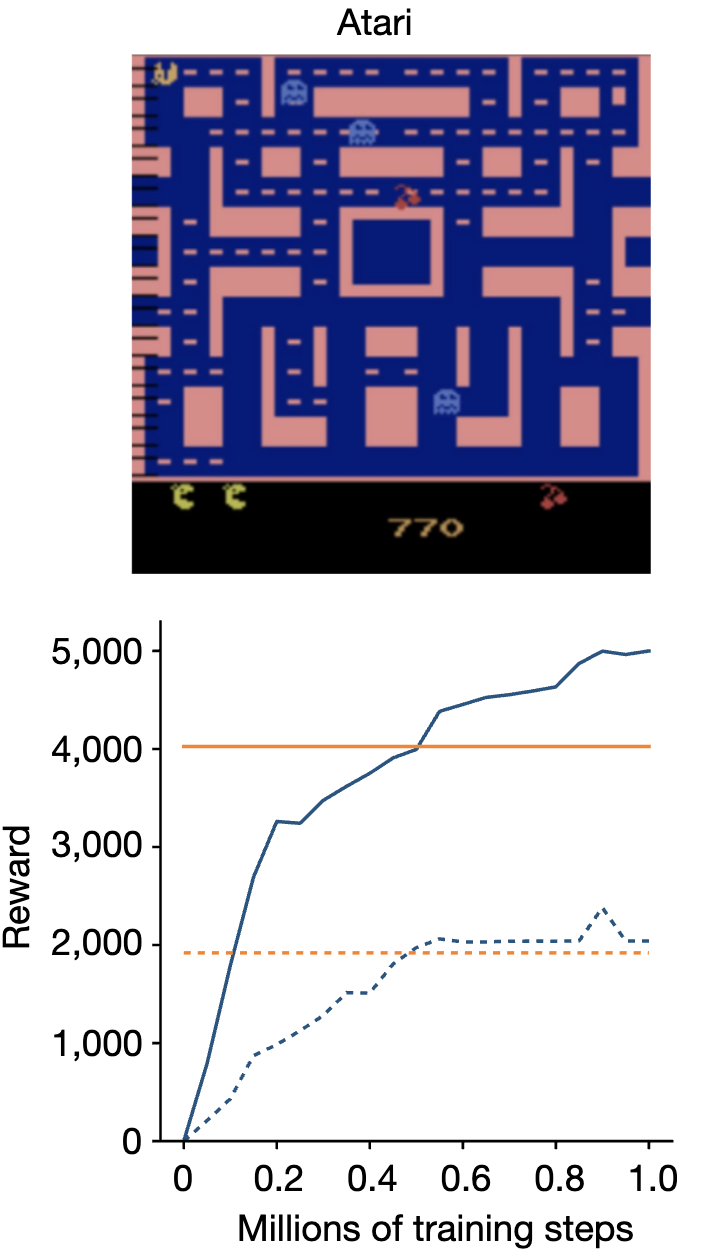
\includegraphics[height= 4.0in]{\images/muzeroatari}}

{\huge
  These are human normalized scores averaged over all 57 Atari games.  The orange line is the previous state of the art system.  Solid lines are average scores and dashed lines are median scores.
}


\slide{AlphaStar}

Grandmaster level in StarCraft II using multi-agent reinforcement learning, Nature Oct. 2019, Vinyals et al.

\vfill
StarCraft:

\begin{itemize}
\item Players control hundreds of units.

\vfill
\item Individual actions are selected from $10^{26}$ possibilities (an action is a kind of procedure call with arguments).

\vfill
\item Cyclic non-transitive strategies (rock-paper-scissors).

\vfill
\item Imperfect information --- the state is not fully observable.
\end{itemize}

\slide{The Paper is Vague}

It basically says the following ideas are used:

A policy gradient algorithm, auto-regressive policies, self-attention over the observation history,L STMs, pointer-networks, scatter connections,
replay buffers, asynchronous advantage actor-critic algorithms, TD($\lambda$) (gradients on value function Bellman error), clipped importance sampling
(V-trace), a new undefined method they call UPGO that ``moves policies toward trajectories with better than average reward'', a value function
that can see the opponents observation (training only), a ``$z$ statistic'' stating a high level strategy, 
supervised learning from human play, 
a ``league'' of players (next slide).

\slide{The League}

The league has three classes of agents: main (M), main exploiters (E), and league exploiters (L).  M and L play against everybody.
E plays only against M.

\slide{A Rube Goldberg Contraption?}

\centerline{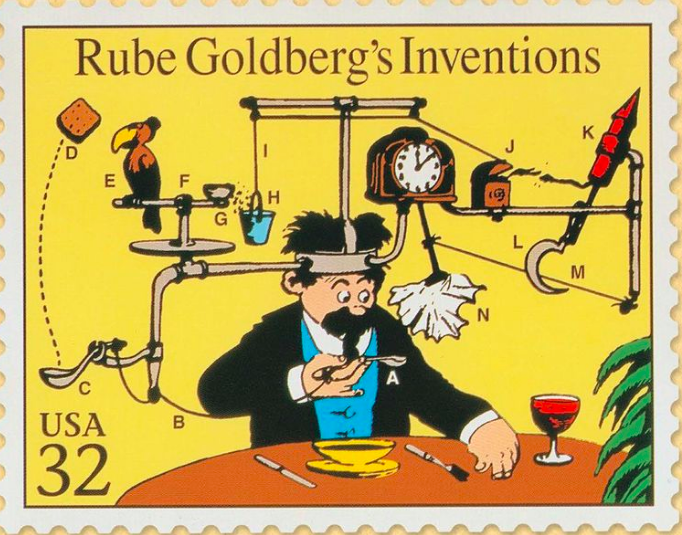
\includegraphics[height = 5in]{\images/Goldberg}}

\slide{Video}

https://www.youtube.com/watch?v=UuhECwm31dM

\slide{Cicero: Diplomacy}

{\bf Human-level play in the game of Diplomacy by combining language models with strategic reasoning}, (Meta, November 2022)

\vfill
Players engages in secret negotiaions to conspire to take over the world.

\vfill
\centerline{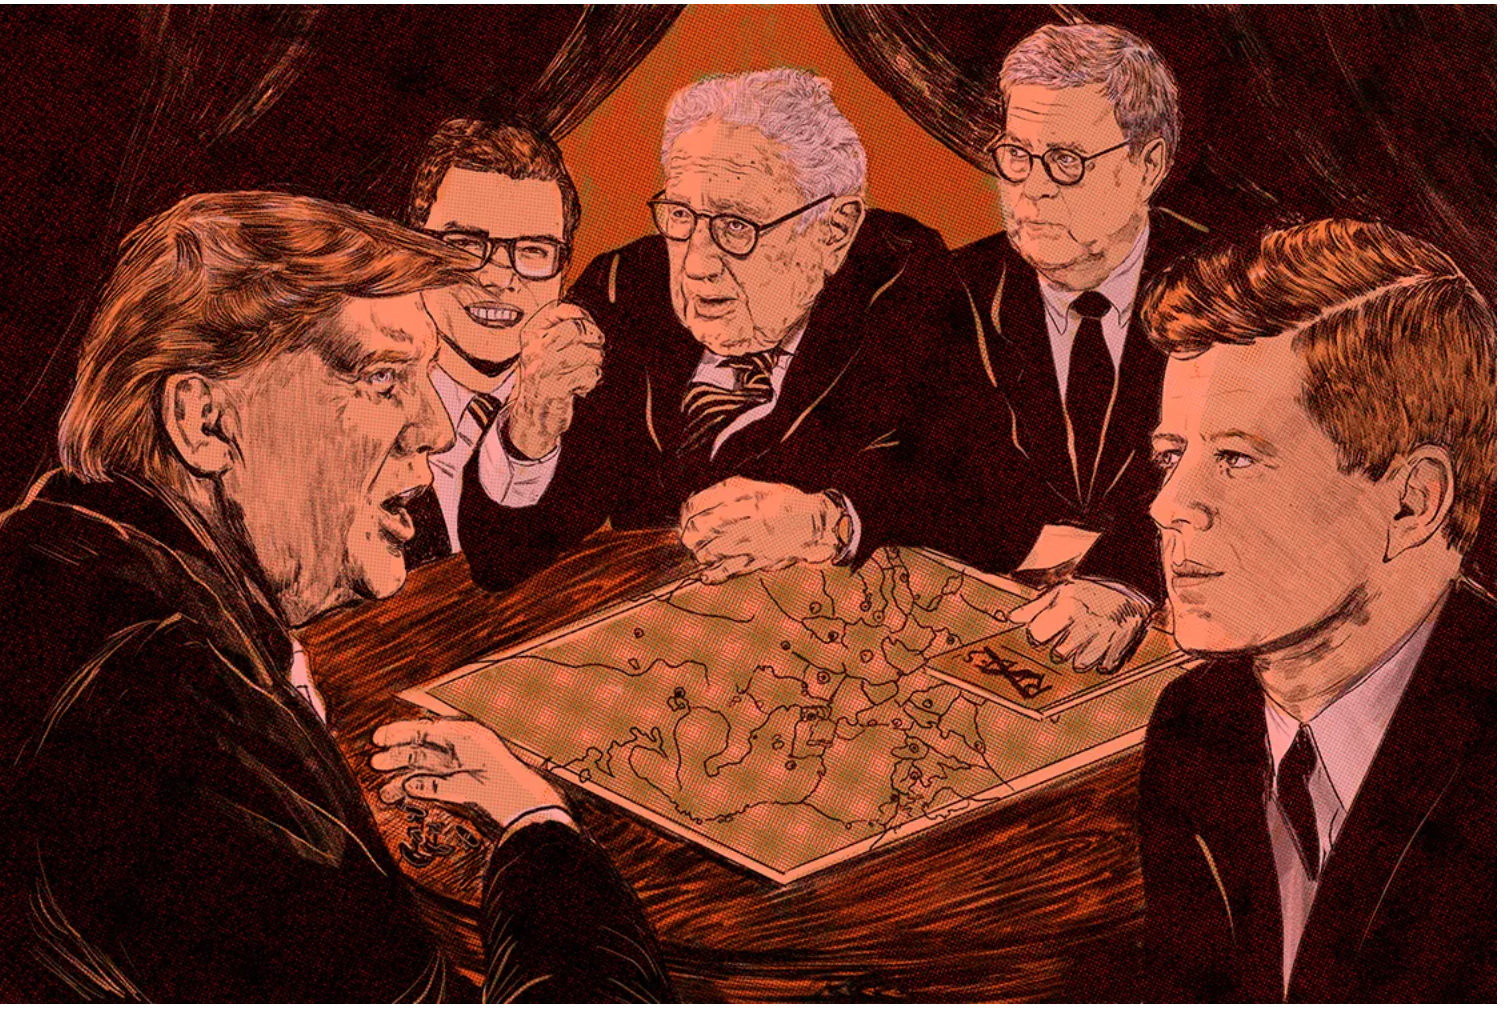
\includegraphics[width = 4.0in]{\images/Diplomacy02}\hfill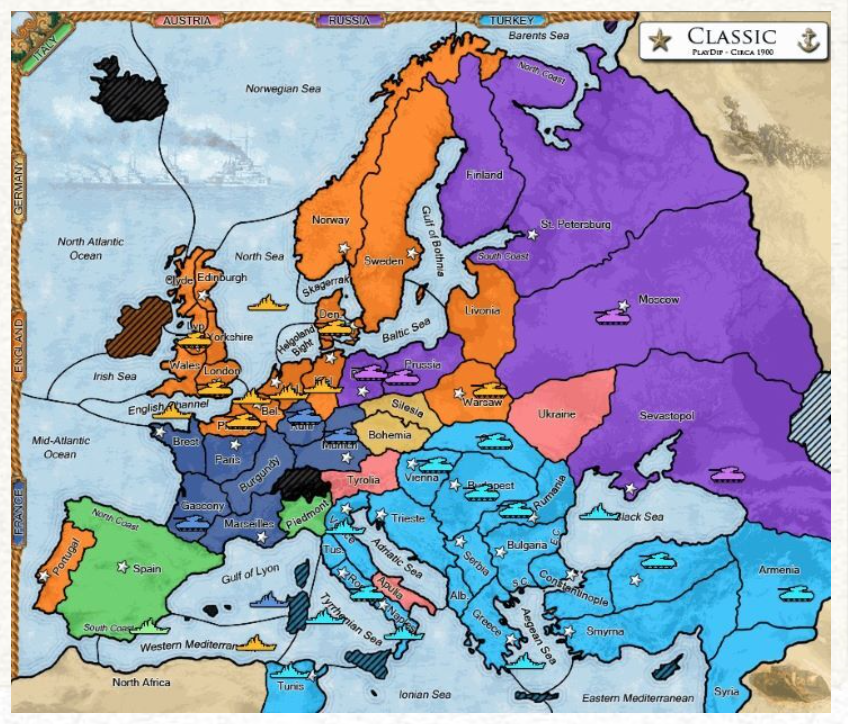
\includegraphics[width = 3.0in]{\images/Diplomacy01}}

\slide{Cicero: Diplomacy}

\vfill
\centerline{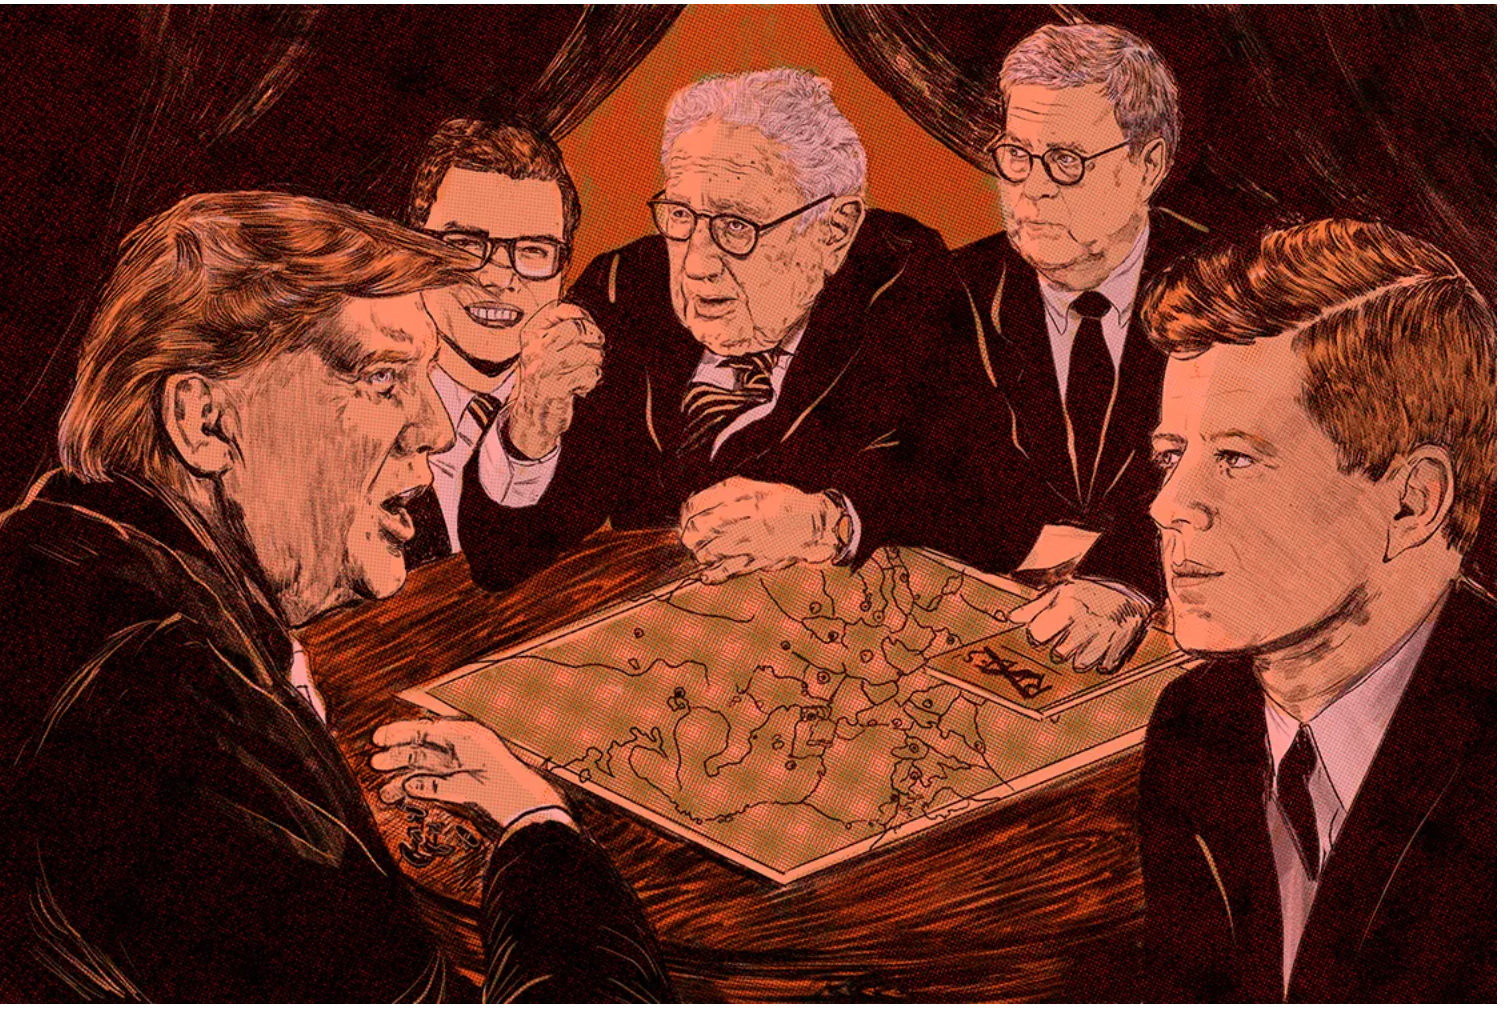
\includegraphics[width = 3.0in]{\images/Diplomacy02}\hspace{4em}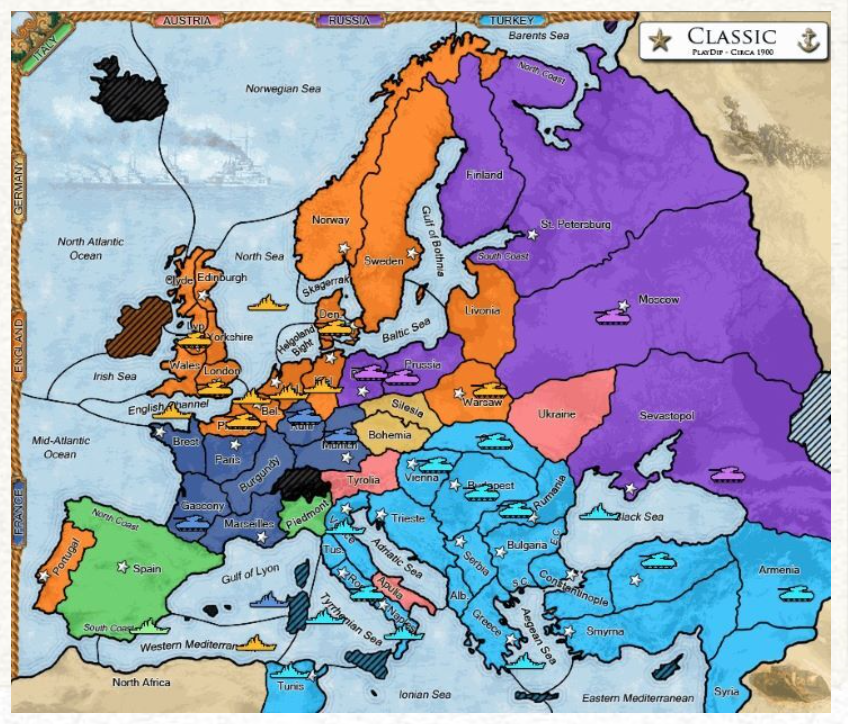
\includegraphics[width = 2.0in]{\images/Diplomacy01}}

\vfill
The play consists of a sequence of ``turns''.  In each turn each player converses with the others using a private messaging system.  After some time the messaging ends and each player submits orders to their generals.  The orders are revealed simultaneously. Promises can be broken.


\slide{Cicero: Diplomacy}

Cicero is an AI agent that plays Diplomacy with humans.  It is rated in the top 10\% of human players.


\slide{Action Planning}

We define the action of a player to be the set of orders that the player gives to their generals at the end of the turn.

\vfill
Cicero plans its actions for the current turn and generates ``beliefs'' about the actions of the other players (mathematically equivalent
to stochastic policies for the other players).  Messages are generated from Cicero's planned actions and beliefs.  The planned actions
and beliefs can evolve during negotiation.

\slide{A Value Function}

We seek a winning strategy (policy) for the agent Cicero.

\vfill
A choice of actions $a_1,\ldots,a_n$ for all the players determines the next board state.

\vfill
Cicero trains a value function that assigns a value $V_q(b)$ giving an estimate of the value that player $q$ receives 
for board position $b$.

\vfill
As policies are trained and estimated, the value function can be trained with standard methods --- Bellman error and replay buffers.

\slide{Correlated Nash Equilibria}

\vfill
At the end of negotiation it is natural to search for policies, $\pi_1,\ldots,\pi_n$ conditioned on the negotiation
that form a (correlated) Nash equilibrium.

\vfill
This mean that each policy is a ``best response'' to other players policies where all policies are conditioned
on the negotiation.

\vfill
It is ``correlated'' because the actions of two players are not independent when they can negotiate an agreement.

\slide{Training Data}

Cicero is trained on a dataset of 12,901,662 games from WebDiplomacy including messages exchanged between players. (webDiplomacy deidentified Player accounts).


\newcommand{\act}{\mathrm{act}}
\newcommand{\mess}{\mathrm{mess}}
\newcommand{\im}{\mathrm{im}}

\slide{An Imitation Model of Action Prediction}

We want to predict actions during negotiation.

\vfill
$$\im^* = \argmin_\im\;E_{(x_p,a_q) \sim \train}\left[-\ln P_\im(a_q|x_p)\right]$$

\vfill
Here $p$ and $q$ are players. $x_p$ is taken from a time in a negotiation and
consists of all past board positions and the previous messages in this negotiation visible to player $p$.
$a_q$ is the action taken at the end of that round by player $q$.

\vfill
If $q = q$ this is an imitation action policy for $p$.

\vfill
If $q \ne p$ this is $p$'s imitation belief about $q$.

\slide{piKL}

Let $c$ denote player Cicero.

\vfill
Before sending each negotiation message Cicero samples 30 actions for each player $q$
from the imitation action predictions $P(a_q|x_c)$ (including actions for Cicero).

\vfill
Cicero then optimizes policies $\pi_1,\ldots,\pi_n$ according to a piKL best-response objective
where $\pi_{-p}$ is the collection of policies other than $\pi_p$.

$$\pi_p^* = \argmax_{\pi_p}\;V(\pi_p,\pi_{-p}) - \lambda KL(\pi_p,P_\im(a_p|x_c)$$



\slide{Imitation Message Generation}

Cicero has a model $P_\mess(y|s,r,a_s,a_r,x_s)$ where
where $y$ is the English text of the message, $s$ is the message sender, $r$ is the message recipient,
$a_s$ is the action taken by the message sender and $a_r$ is the action
taken by the message receiver at the end of the turn (in the future).

\vfill
$x_s$ consists of all past board positions and the previous messages visible to the sender in the current negotiation.

\slide{Imitation Message Generation}

{\huge
$$\mess^* = \argmin_\mess\;E_{\{(x,s,r,y,a_s,a_r) \sim \train\}} \left[-\ln P_\mess(y|s,r,a_s,a_r,x_s)\right]$$
}

\slide{An Imitation Agent}

\vfill
$$P_\im(y|s,r,x_s) = E_{\{a_s,a_r \sim P_\act(a_s,a_r|s,r,x_s)\}}\;P_\mess(y|s,r,a_s,a_r,x_s)$$


\vfill
In Cicero the imitation model is combined with a planning model.

\slide{Action Planning}

\slide{??}


\vfill




\vfill
The trained policies come two versions --- an expensive version conditioned on the board state plus dialogue,
and a cheaper version conditioned just on the board state.

\vfill








\slide{Selecting the End Of Turn Action}

For each turn Cicero first decides on its final action (the orders that it will give at the end of the turn) and then
generates messages 

\vfill
The sends messages specified by intents.  This is done by deciding on an ``action'' which specifies all of the orders
that the agent will actually give.specifying all of the payers orders
where $x$ is as before (the history of board positions, and the history of messages before the message to be generated.



\vfill
A message prediction model $P_\mess(y|A,B,I,x)$ where $A$ and $B$ are two players, $y$ is a message from $A$ to $B$, $I$ is a (latent) ``intent'' of the message, and
$x$ includes the history of board states the message and the messaged in the current turn occuring before this message.

\vfill
{\bf Step 2:} They get a base model --- a 2.7B parameter transformer
model pre-trained on text from the internet.

\vfill
{\bf Step 3:} The base model is fine-tuned to predict messages from the board state, the previous messages negotiation in the WebDiplomacy dataset.

\vfill
$\vdots$

\slide{{\bf Step 4:} Inferring Intents}

The set of legal orders for any position 

A an ``intent'' for a message from player $A$ to player $B$ is a set of orders for $A$ and a set of orders for $B$ 

These steps are explained in more detail below.

\vfill
{\bf Step 4:} They train a model to infer an ``intent'' of each message based on the orders that followed in game move.
\vfill
{\bf Step 5:} They train a model annotate messages with the intent of the message.

\vfill
{\bf step 6:} 

\slide{Cicero is an Elaborate System}

\centerline{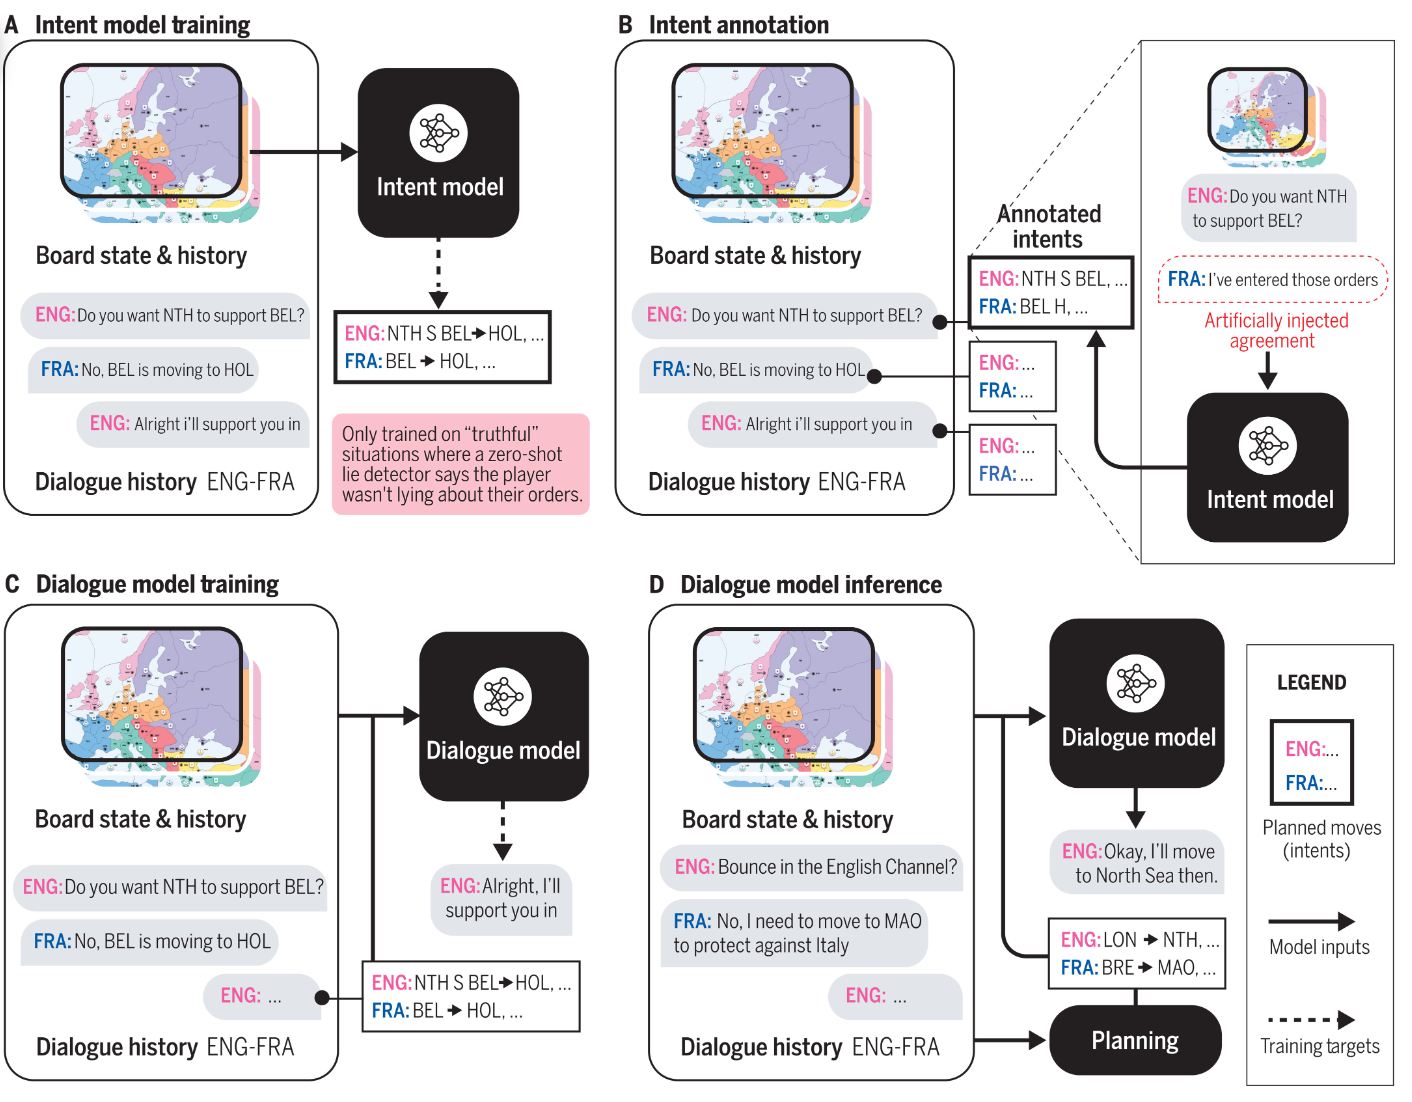
\includegraphics[width = 6in]{\images/Diplomacy3}}


\slide{Cicero: Diplomacy}

Cicero is an AI agent that plays Diplomacy with humans.  It is rated in the top 10\% of human players.

\vfill

\centerline{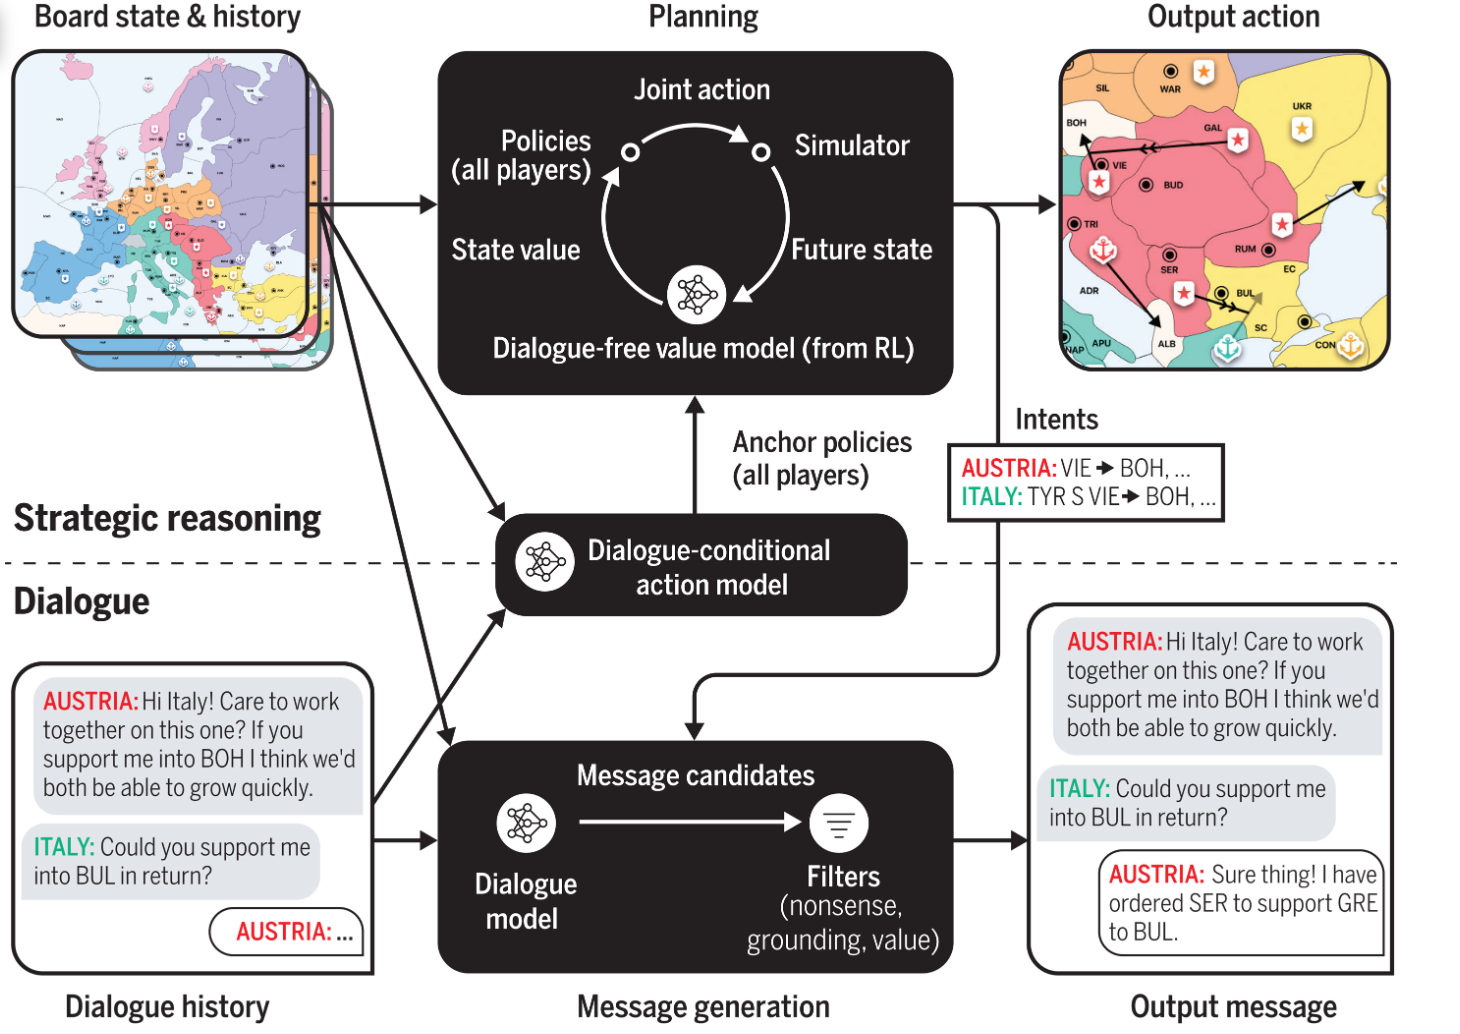
\includegraphics[height = 4.0in]{\images/Diplomacy1}}


\slide{END}

}
\end{document}
